\begin{figure}[htbp]
\centering
\begin{tikzpicture}[x=1cm,y=1cm]
\node[anchor=south west,inner sep=0] at (0,0) {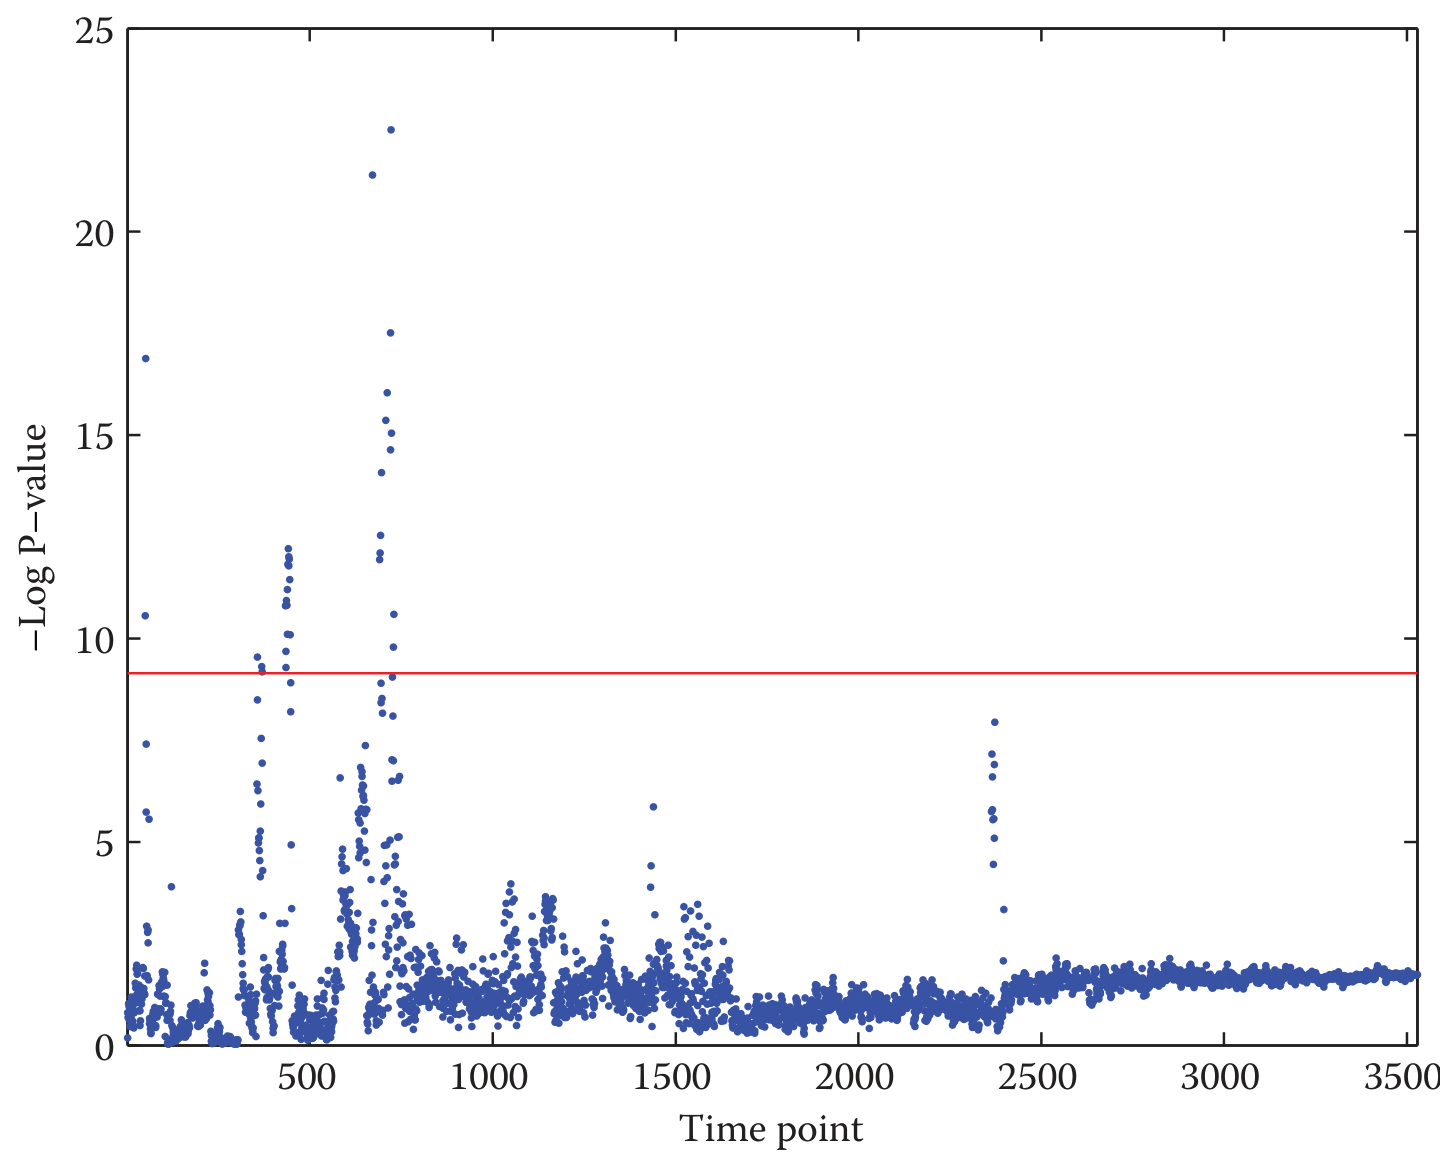
\includegraphics[width=13.8cm]{figures/ch03_fig21_data.png}};
\fill[white] (6.4706,0.0630) rectangle (8.3076,0.4906);
\node[font=\small,rotate=0,inner sep=0] at (7.3891,0.2768) {时间点};
\fill[white] (0.1183,4.8410) rectangle (0.5591,7.0798);
\node[font=\small,rotate=90,inner sep=0] at (0.3387,5.9604) {$-\log P$ 值};
\end{tikzpicture}
\origfig{21}{整夜各时间点，使用 MLMT 检验基因 TMEM50B 内全部 SNP 与血氧饱和度关联所得的 $P$ 值随时间 $t$ 的变化。}
\label{fig:ch03-21}
\end{figure}
